\documentclass[12pt, titlepage]{article}

\usepackage{fullpage}
\usepackage[round]{natbib}
\usepackage{multirow}
\usepackage{booktabs}
\usepackage{tabularx}
\usepackage{graphicx}
\usepackage{float}
\usepackage{hyperref}
\usepackage{siunitx}
%\usepackage{placeins} For float barrier but doesn't seem necessary anymore
\hypersetup{
    colorlinks,
    citecolor=blue,
    filecolor=black,
    linkcolor=red,
    urlcolor=blue
}


%%% Comments

\usepackage{color}

\newif\ifcomments\commentstrue %displays comments
%\newif\ifcomments\commentsfalse %so that comments do not display

\ifcomments
\newcommand{\authornote}[3]{\textcolor{#1}{[#3 ---#2]}}
\newcommand{\todo}[1]{\textcolor{red}{[TODO: #1]}}
\else
\newcommand{\authornote}[3]{}
\newcommand{\todo}[1]{}
\fi

\newcommand{\wss}[1]{\authornote{blue}{SS}{#1}} 
\newcommand{\plt}[1]{\authornote{magenta}{TPLT}{#1}} %For explanation of the template
\newcommand{\an}[1]{\authornote{cyan}{Author}{#1}}

%%% Common Parts

\newcommand{\progname}{ProgName} % PUT YOUR PROGRAM NAME HERE
\newcommand{\authname}{Team \#, Team Name
\\ Student 1 name
\\ Student 2 name
\\ Student 3 name
\\ Student 4 name} % AUTHOR NAMES                  

\usepackage{hyperref}
    \hypersetup{colorlinks=true, linkcolor=blue, citecolor=blue, filecolor=blue,
                urlcolor=blue, unicode=false}
    \urlstyle{same}
                                

\newcommand{\progname}{SmartServe} % PUT YOUR PROGRAM NAME HERE
\newcommand{\authname}{Team 21, StoneCap Solutions
\\ Max Turek $turekm$
\\ Ryan Were $werer$
\\ Sam Nusselder $nusselds$
\\ Peter Minbashian $minbashp$
\\ David Bednar $bednad1$} % AUTHOR NAMES                  

\usepackage{hyperref}
    \hypersetup{colorlinks=true, linkcolor=blue, citecolor=blue, filecolor=blue,
                urlcolor=blue, unicode=false}
    \urlstyle{same}
\newcounter{acnum}
\newcommand{\actheacnum}{AC\theacnum}
\newcommand{\acref}[1]{AC\ref{#1}}

\newcounter{ucnum}
\newcommand{\uctheucnum}{UC\theucnum}
\newcommand{\uref}[1]{UC\ref{#1}}

\newcounter{mnum}
\newcommand{\mthemnum}{M\themnum}
\newcommand{\mref}[1]{M\ref{#1}}

\begin{document}

\title{System Design for \progname{}} 
\author{\authname}
\date{\today}

\maketitle

\pagenumbering{roman}

\section{Revision History}

\begin{tabularx}{\textwidth}{| s | s | s | X |}
        \toprule
        \textbf{Version} & \textbf{Date} & \textbf{Developer(s)} & \textbf{Change(s)}\\
        \midrule
         & & Max Turek & \\
         & & Ryan Were & \\
        0 & 01/18/23 & Sam Nusselder & Initial Draft\\
         & & Peter Minbashian & \\ 
         & & David Bednar & \\ 
        \bottomrule
        \hline
        1.0 & 04/04/23 & Max Turek & Changes to the scope, additions to component diagram, changes to requirements to fit final product, added new images for the web app and physical machine, changed the final communication protocol
        \hline
\end{tabularx}

\newpage

\section{Reference Material}

\subsection{Abbreviations and Acronyms}
Please refer to \href{https://github.com/purefisher/Smart-Serve/blob/main/docs/SRS/SRS.pdf}{SRS} 
%\renewcommand{\arraystretch}{1.2}
%\begin{tabular}{l l} 
%  \toprule		
%  \textbf{symbol} & \textbf{description}\\
%  \midrule 
%  \progname & Explanation of program name\\
%  \wss{...} & \wss{...}\\
%  \bottomrule
%\end{tabular}\\

\newpage

\tableofcontents

\newpage

\listoftables

\listoffigures

\newpage

\pagenumbering{arabic}

\section{Introduction}
The detailed design document is one of three design documents that encompasses the entire design of the Smart Serve system. Please refer to \href{https://github.com/purefisher/Smart-Serve/blob/main/docs/Design/DetailedDesign.pdf}{DetailedDesign} and \href{https://github.com/purefisher/Smart-Serve/blob/main/docs/Design/DetailedDesi.pdf}{Software Architecture} for further design information.
\section{Purpose}
The purpose of this design documentation, is to decompose the Smart Serve system into different components for design implementation and presentation. These components include the user interface, the hardware and electrical design and finally any communication protocol design. 

\section{Scope}
The setting of the Smart Serve system is intended to be used within a bar/pub setting by patrons or by a user in their home. Users will have the option to order drinks using an internet connected device by heading to the Smart Serve URL and accessing the web application. The user will then login and have the option to order a drink of their choosing on the menu. Once ordered the Smart Serve machine will begin creating the drink and once finished alert the user that the drink has been finished. The user will then retrieve their drink from the machine and the next user will have the option to order or could have already ordered thus being placed in a queue. 
\begin{figure}[H]
    \centerline{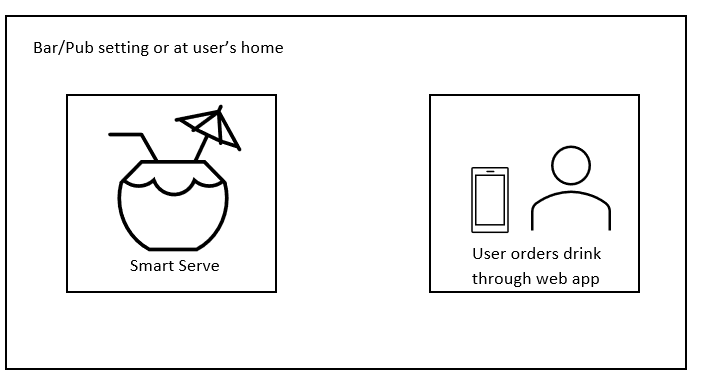
\includegraphics[scale=.5]{systemboundary.png}}
    \caption{System Boundary}
    \label{fig}
\end{figure}

\section{Project Overview}

\subsection{Normal Behaviour}
Smart Serve is intended to be used in within the environment of a bar or at a user's dwelling. During normal operation, user's will be able to access the web application through entering the link or scanning the QR code. On the web application users will be able to order cocktails from a variety of given options, which will then be created autonomously by the Smart Serve system. Once the drink has been completed, the user will be notified via the web app, and they will then be asked to retrieve their cocktail. This system will reduce the burden on bartenders and provide quick service to customers needing a drink.

\subsection{Undesired Event Handling}
Undesired events are bound to happen, for example the wifi/power turning off or perhaps a user tampering with the physical components of the system. In these scenarios, we plan on creating a "safe state" for our system that upon undesired events, it can enter into while avoiding any potential hazards. An operator will be notified to check the system after an undesired event, in order to resume the system into normal operation.

\subsection{Component Diagram}
\begin{figure}[H]
    \centerline{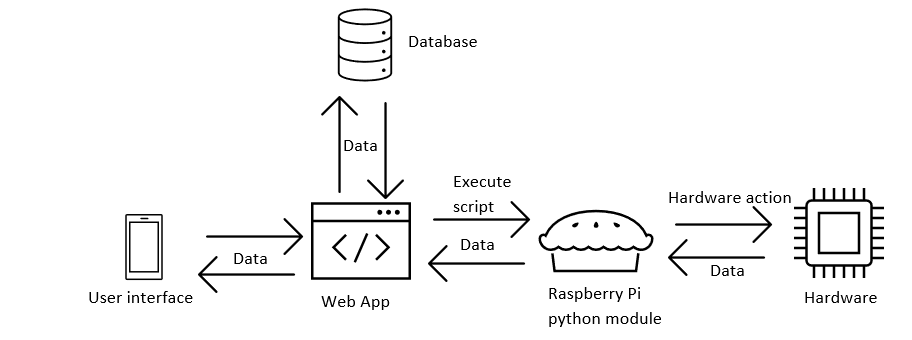
\includegraphics[scale=.5]{componentdiagram.png}}
    \caption{Component Diagram}
    \label{fig}
\end{figure}
The component diagram decomposes each independent component of our system and how they interact with each other. The web application, is the only access point for the user for drink ordering. They must access this from an internet connected device. The web app queries the database to retrieve past drink orders, drink ingredients and users login information. The web app spawns a process to run a python script that controls the hardware of the machine. The python script will send a done signal to the web app alerting that will allow the web app to process the next drink order in the queue and this cycle repeats. 

\subsection{Connection Between Requirements and Design} \label{SecConnection}

%\wss{The intention of this section is to document decisions that are made
%  ``between'' the requirements and the design.  To satisfy some requirements,
%  design decisions need to be made.  Rather than make these decisions implicit,
%  they are explicitly recorded here.  For instance, if a program has security
%  requirements, a specific design decision may be made to satisfy those
%  requirements with a password.}
\subsubsection{Quality requirements of the entire system}
    \noindent\textbf{QR1.} Smart Serve must be robust\\ 
    \indent\textbf{Design consideration:} Smart Serve will be created out of structurally sound materials and will be designed to be durable after much use.
\subsubsection{Look and Feel Requirements}
    \noindent\textbf{LFR1.} The web app must be intuitive and visually appealing \\
    \indent\textbf{Design consideration:} Web app designed for minimal clicks needed to use.\\\\
    \textbf{LFR2.} Smart Serve must have all electrical and mechanical components concealed \\
    \indent\textbf{Design consideration:} All electrical and mechanical components are concealed by designing a wood frame around them.

\subsubsection{Usability and Humanity Requirements}
    \textbf{Ease of use}\\
        \noindent\textbf{UHR1.} Smart Serve must serve the drink at a height that is easy to grab for an average adult \\
        \indent\textbf{Design consideration:} Smart Serve is designed to be set on a table to ensure it is easy for the users to grab their drinks.\\\\
        \textbf{UHR2.} Smart Serve must make grabbing the drink easy for the user, without blockages or inconveniences\\
        \indent\textbf{Design consideration:} Smart Serve is designed to be forward facing and have nothing in front of where the finished drink will be.\\\\
        \textbf{UHR4.} The web app must make it easy to navigate and select drinks\\
        \indent\textbf{Design consideration:} The web app is designed to have a very intuitive menu system that shows images and drink names for the drinks that are available to order.\\\\
    \textbf{Ease of learning}\\
        \noindent\textbf{UHR5.} Finding and gaining access to the web app must be easy \\
        \indent\textbf{Design consideration:} The web app will be linked to a QR code which can be accessed with any phone. Any electronic device can search up the URL to order from the web app too.

\subsubsection{Performance Requirements}
    \textbf{Speed requirement}\\
        \noindent\textbf{PR1.} The drink must be ready and served within 60 seconds of when the drink began to be made \\
        \indent\textbf{Design consideration:} All drinks created are made in the same proportions and using the same pumps with the same flow rates allowing every drink to be created in 60 seconds or less.\\\\
        \textbf{PR2.} The web app must be highly responsive to user inputs \\
        \indent\textbf{Design consideration:} The web app is designed to respond quickly to any and all user inputs.\\\\
        \textbf{PR3.} The web app must add a users order to the queue of orders within 5 seconds of ordering \\
        \indent\textbf{Design consideration:} The web app adds the users order to the queue quickly be calling a function to update the queue.\\\\
    \textbf{Safety critical requirement}\\
        \noindent\textbf{PR4.} Smart Serve must not release more than 1.1x the amount of expected alcohol \\
        \indent\textbf{Design consideration:} The pumps flow rate specifications are very close to the measured flow rate. Taking accurate time measurements to ensure that the alcohol added to the drink is not more than 1.1x will ensure this requirement is met.\\\\
        \noindent\textbf{PR5.} Smart Serve must be able to measure drink ingredients within 10\% of the expected value \\
        \indent\textbf{Design consideration:} The pumps flow rate specifications are very close to the measured flow rate. Taking accurate time measurements to ensure that the drink ingredients added to the drink are within 10\% of the expected value will ensure this requirement is met.\\\\
    \textbf{Reliability and availability requirement}\\
        \noindent\textbf{PR6.} Smart Serve must be able to create the correct drink every time as long as it has the correct ingredients \\
        \indent\textbf{Design consideration:} The ingredient containers and pumps are numbered and will match the numbering in the code to ensure the proper ingredient is always added to the drink.\\\\
    \textbf{Capacity requirement}\\
        \noindent\textbf{PR7.} Smart Serve must be able to store up to 5 ingredients \\
        \indent\textbf{Design consideration:} Smart Serve has been designed to hold five 2L pop bottles and have five separate pumps allowing for 5 ingredients.\\\\
        \textbf{PR8.} Smart Serve must be able to store up to 1 liters of each ingredient \\
        \indent\textbf{Design consideration:} The ingredient containers are 2L each in size.

\subsubsection{Operational and Environmental Requirements}
    \textbf{Expected physical environment}\\
        \noindent\textbf{OER1.} Smart Serve must not be exposed to rain or poor weather \\
        \indent\textbf{Design consideration:} Smart Serve is designed to have all the important components fully enclosed. Also, Smart Serve is recommended for indoor use only.\\\\
        \textbf{OER2.} Smart Serve must be placed upright on a flat surface \\
        \indent\textbf{Design consideration:} Smart Serve has a flat base and is designed to sit upright on a flat surface.\\\\
    \textbf{Expected technological environment}\\
        \noindent\textbf{OER4.} Smart Serve must have access to wifi \\
        \indent\textbf{Design consideration:} Smart Serve has an ethernet cable built into it and can be connected to wifi through the raspberry pi or via wireless.\\\\
        \textbf{OER5.} Smart Serve must have access to electricity \\
        \indent\textbf{Design consideration:} Smart Serve has all the required plugs come out the back together to make it simple to be plugged into a wall outlet.\\\\
        \textbf{OER6.} The user must have internet access to the same wifi network as Smart Serve and a device to access the web app \\
        \indent\textbf{Design consideration:} Smart Serve is intended to be used indoors in an environment that has internet access, furthermore user must be connected to the same network otherwise they will not be able to connect. WiFi details will be viewable/accessible to user.\\\\
    \textbf{Partner applications}\\
        \noindent\textbf{OER7.} Smart Serve must be equipped with a cup to serve a drink \\
        \indent\textbf{Design consideration:} Smart Serve is compatible with basic red solo cups that will be available at the location where it is used.

\subsubsection{Maintainability and Support Requirements}
    \textbf{Maintainability}\\
        \noindent\textbf{MSR1.} Smart Serve should be cleaned at least once every day \\
        \indent\textbf{Design consideration:} Smart Serve is designed so the components that need to be cleaned can be easily accessed for cleaning. There is a clean lines option on the web app allowing the operator to run water through the lines.\\\\
        \textbf{MSR2.} Smart Serve must be restocked with new ingredients to be able to serve drinks \\
        \indent\textbf{Design consideration:} Smart Serve is designed to have 2 doors open at the back that are connected to the ingredient storage area so the operator can easily restock new ingredients.\\\\
    \textbf{Special Maintenance Conditions} \\
        \noindent\textbf{MSR3.} No electronic or water sensitive components of Smart Serve can get wet during cleaning \\
        \indent\textbf{Design consideration:} Smart Serve is designed so the electronic and water sensitive components are separated from the areas that need to be cleaned.\\\\
        \textbf{MSR4.} The operator must add the ingredients to the web app when Smart Serve is restocked \\
        \indent\textbf{Design consideration:} The web app is designed so the operator can simply go to the operator login side of the web app and intuitively add the restocked ingredients.\\\\
    \textbf{Portability}\\
        \noindent\textbf{MSR5.} Smart Serve must be modular and easy to transport \\
        \indent\textbf{Design consideration:} Smart Serve is designed to be one piece and a cube-like design.\\\\
        \textbf{MSR6.} Smart Serve must be under 100 pounds \\
        \indent\textbf{Design consideration:} Smart Serve is designed to weigh under 100 pounds after all the components are added.

\subsubsection{Security Requirements}
    \noindent\textbf{SR1.} The users personal information must be secure \\
    \indent\textbf{Design consideration:} The database is encrypted and password protected, removing access from anyone but admin.\\\\
    \textbf{SR2.} Communication between the web app and Smart Serve must be secure \\
    \indent\textbf{Design consideration:} Communication between the web app and Smart Serve will be done on a separate secure server.\\\\
    \textbf{SR3.} The operator must be responsible for correctly operating the machine and restocking ingredients \\
    \indent\textbf{Design consideration:} Smart Serve is designed for easy operator use for restocking ingredients.\\\\
    \textbf{SR4.} The user must provide identification and be of drinking age to order and receive a drink from Smart Serve \\
    \indent\textbf{Design consideration:} In bar settings, anyone having access to the drink machine is already assumed to have shown identification.

\subsubsection{Cultural and Political Requirements}
    \noindent{Not applicable} 
\subsubsection{Legal Requirements}
    \noindent\textbf{LR1.} Smart Serve must only be used in countries where alcohol is legal \\
    \indent\textbf{Design consideration:} Smart Serve will only be manufactured sold in countries where alcohol is legal.\\\\
    \textbf{LR2.} Smart Serve must not produce a drink that is consumed by persons under the drinking age \\
    \indent\textbf{Design consideration:} Only people of legal drinking age will have access to Smart Serve.\\\\
    \textbf{LR3.} The owner of Smart Serve is liable for all drinks served \\
    \indent\textbf{Design consideration:} The operator of Smart Serve is liable for all drinks served.

\subsubsection{Health and Safety Requirements}
    \noindent\textbf{HSR1.} Smart Serve or the operator must not serve a drink to someone who is dangerously intoxicated \\
    \indent\textbf{Design consideration:} The operator will ensure that anyone who is dangerously intoxicated will not receive any more drinks from Smart Serve.\\\\
    \textbf{HSR2.} Smart Serve should not be operational near unsupervised persons under the drinking age \\
    \indent\textbf{Design consideration:} Smart Serve will only be available to the operator by being kept in a secure location.\\\\
    \textbf{HSR3.} Smart Serve or the operator must not serve more than 2 drinks per hour to one user\textsuperscript{[1]} \\
    \indent\textbf{Design consideration:} The web app ensures that the same person cannot order more than 2 drinks per hour.\\\\
    \textbf{HSR4.} No electrical components can come into contact with any fluid \\
    \indent\textbf{Design consideration:} Smart Serve is designed to keep all electrical components separated from all liquids.


 \section{System Variables}
Please refer to the \href{https://github.com/purefisher/Smart-Serve/blob/main/docs/Design/DetailedDesign.pdf}{DetailedDesign} document for system variables related to the web app and it's internal modules.

\subsection{Monitored Variables}

%\FloatBarrier
\begin{table}[H]
    \begin{tabular}{|p{3cm}|p{3cm}|p{1.5cm}|p{2cm}|p{4cm}|}
       \hline
        \multicolumn{5}{|c|}{Monitored Variables} \\
        \hline
        Variable & Variable Type & Range & Units & Comment(s)  \\ [0.5ex]
        \hline\hline
        M\_cupPresent & Boolean & [0,1] & N/A & If a cup is present \\
        \hline
        M\_cupEmpty & Boolean & [0,1] & N/A & If a cup is empty \\
        \hline
        M\_echo & Input & [0,1] & N/A & Receive echo for ultrasonic sensor \\
        % &  &  &  & \\
        \hline
    \end{tabular}
    \caption{Monitored Variables for Smart Serve System}
    \label{tab: caption}
\end{table}

\subsection{Controlled Variables}

\begin{table}[H]
    \begin{tabular}{|p{3cm}|p{3cm}|p{1.5cm}|p{2cm}|p{4cm}|}
        \hline
        \multicolumn{5}{|c|}{Controlled Variables} \\
        \hline
        Variable & Variable Type & Range & Units & Comment(s)  \\ [0.5ex]
        \hline\hline
        C\_pump & Boolean & [0,1] & N/A & Turns on or off pump \\
        \hline
        C\_motor& Boolean & [0,1] & N/A & Turns on or off turntable motor\\
        \hline
        C\_trigger & Output & [0,1] & N/A & Send trigger for ultrasonic sensor \\
        % &  &  &  & \\
        \hline
        C\_Q_P_u_m_p & Flow Rate & [0,220] & mL/min & Flow rate of the pumps\\
        \hline
        C\_\omega_M_o_t_o_r & Speed & [0,20] & rad/min & Motor speed \\
        \hline
    \end{tabular}
    \caption{Controlled Variables for Smart Serve System}
    \label{tab: caption}
\end{table}

\subsection{Constant Variables}
The following is a list of system variables

\begin{table}[H]
    \begin{tabular}{|p{3cm}|p{3cm}|p{1.5cm}|p{2cm}|p{4cm}|}
        \hline
        \multicolumn{5}{|c|}{Constant Variables} \\
        \hline
        Variable & Variable Type & Range & Units & Comment(s)  \\ [0.5ex]
        \hline\hline
        V_P_o_w_e_r_S_u_p_p_l_y & Voltage & 12 & Volts & Power supply output voltage\\
        \hline
        V_M_o_t_o_r & Voltage & 12 & Volts & Input voltage required for motor\\
        \hline
        V_P_u_m_p & Voltage & 12 & Volts &  Input voltage required for pumps\\
        \hline
        V_U_l_t_r_a_S_o_n_i_c & Voltage & 5 & Volts &  Input voltage required for ultrasonic sensors\\
        \hline
        V_R_e_l_a_y_M_o_d_u_l_e & Voltage & 5 & Volts &  Input voltage required for relay module\\
        \hline
        % &  &  &  & \\
        \hline
    \end{tabular}
    \caption{Constant Variables for Smart Serve System}
    \label{tab: caption}
\end{table}


\section{User Interfaces}

\begin{figure}[H]
    \centerline{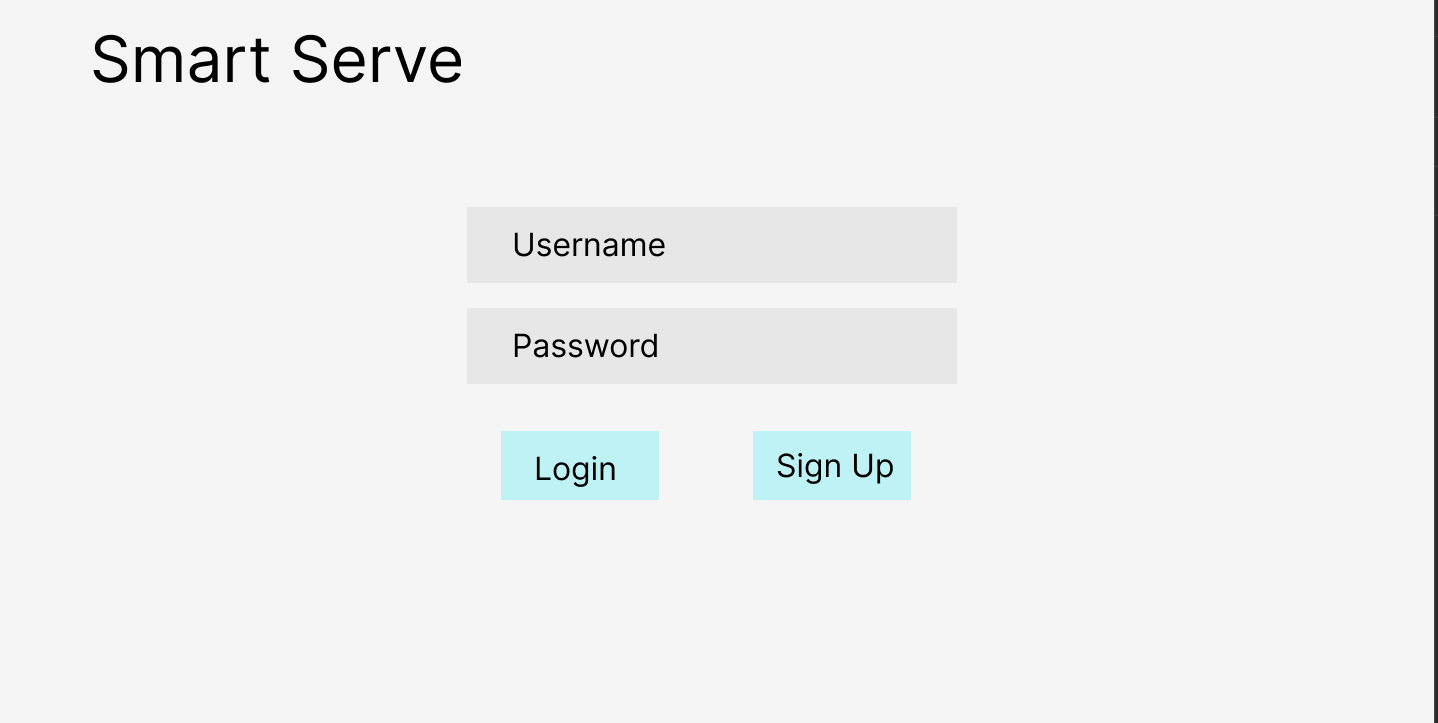
\includegraphics[scale=.5]{Login.png}}
    \caption{Login Page}
    \label{fig}
\end{figure}

\begin{figure}[H]
    \centerline{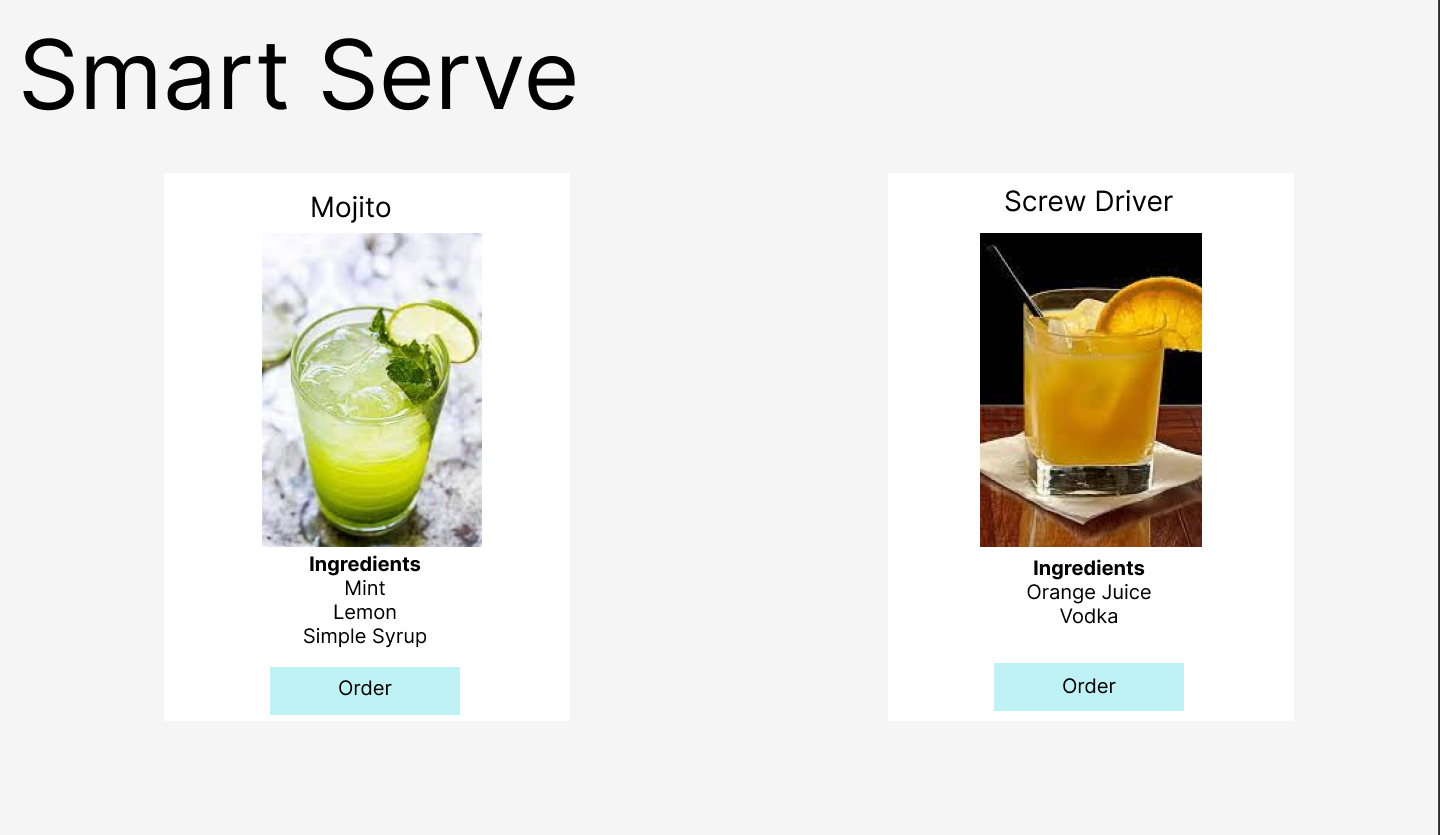
\includegraphics[scale=.5]{Order.png}}
    \caption{Order Page}
    \label{fig}
\end{figure}

\begin{figure}[H]
    \centerline{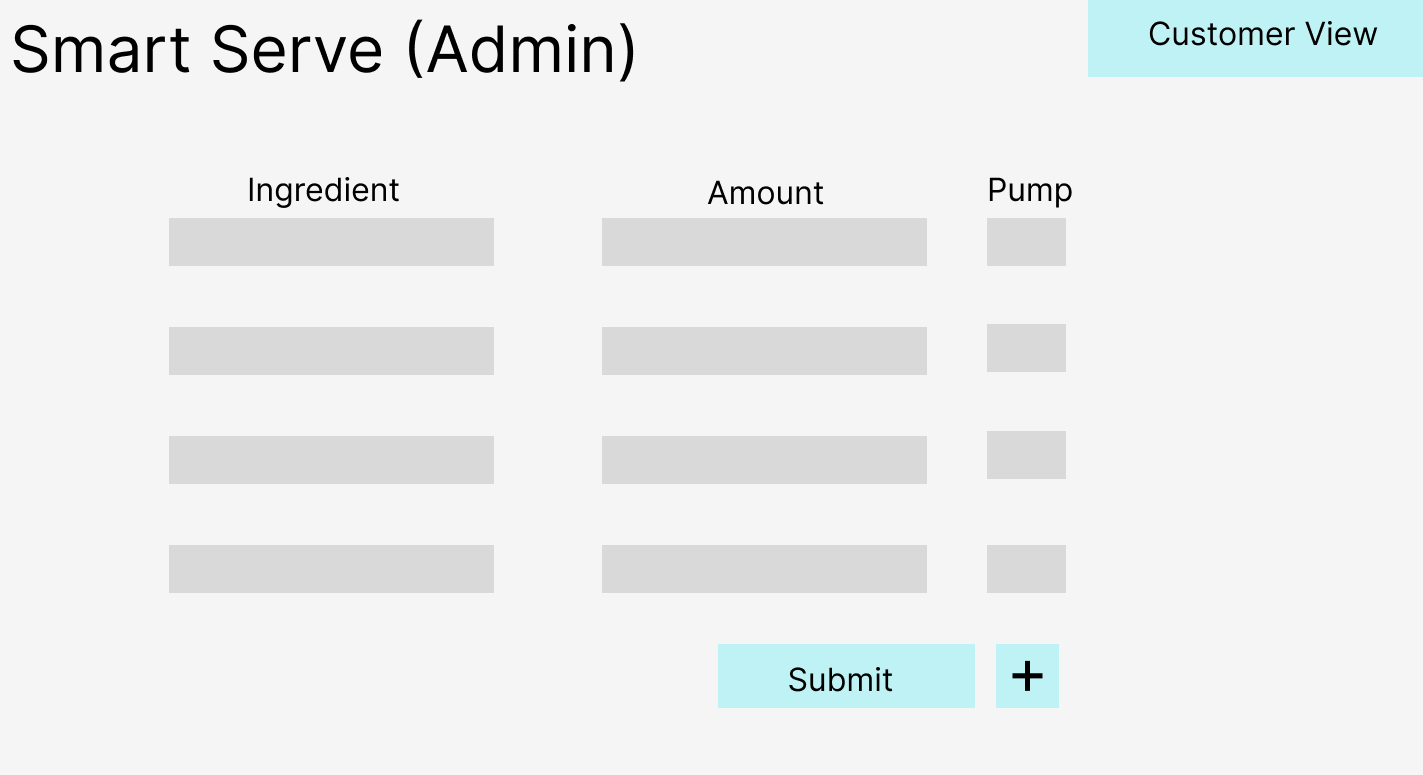
\includegraphics[scale=.5]{Admin.png}}
    \caption{Admin Page}
    \label{fig}
\end{figure}


\section{Design of Hardware}

%\wss{Most relevant for mechatronics projects}
%\wss{Show what will be acquired}
%\wss{Show what will be built, with detail on fabrication and materials}
%\wss{Include appendices as appropriate, possibly with sketches, drawings, CAD, etc}
\subsection{CAD Overview}
\noindent{Figure 6: Smart Serve Overview CAD shows a CAD model of what Smart Serve will look like when completed. It is primarily made out of wood to ensure it is able to support the weight of all the components and because of wood's durability and low cost.}

\begin{figure}[H]
    \centerline{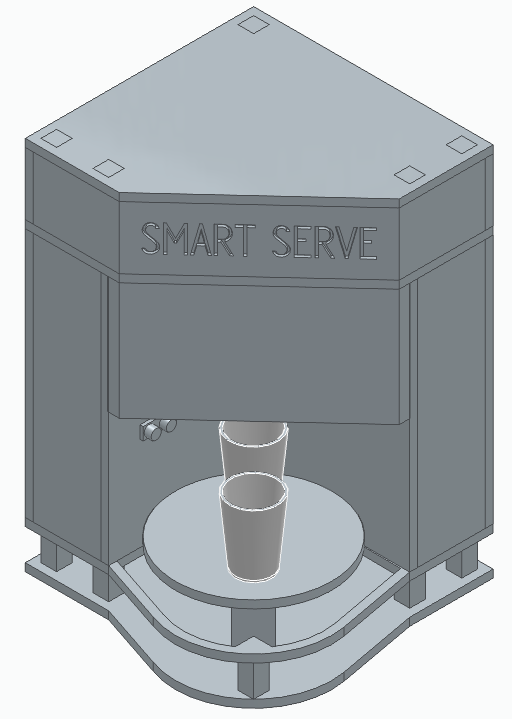
\includegraphics[scale=.5]{Smart Serve Overview CAD.png}}
    \caption{Smart Serve Overview CAD}
    \label{fig}
\end{figure}

\noindent{All the electrical components except the stepper motor are located in the top compartment above the ingredient containers. This is to ensure the electronics and liquids aren't mixed. The stepper motor is located directly below the turntable which should protect it as no liquids will be able to access it. }

\subsection{Bill of Materials}
\noindent{Below is a bill of materials for all the hardware required to build the above CAD model. Note all the electrical components have been included below in section 10.1.}
\begin{table}[H]
    \begin{tabular}{|p{3cm}|p{10cm}|}
       \hline
        \multicolumn{2}{|c|}{Bill of Materials} \\
        \hline
        Number & Item \\ [0.5ex] 
        \hline\hline
        1. & 7 x Wood posts 1" x 1" x 20" long \\
        \hline
        2. & 1 x Wood posts 2" x 2" x 5" long \\
        \hline
        3. & 10 x Wood side boards 0.5" thick x 24" wide x 24" tall \\
        \hline        
        4. & 1 x Wood side board 1" thick x 15" wide x 15" tall \\
        \hline        
        5. & 2 x Draw catch clips \\
        \hline 
        6. & 4 x Hinge fixed pin \\
        \hline        
        7. & 50 x wood screws 1" \\
        \hline        
        8. & 25 x wood screws 2" \\
        \hline
        9. & 10 x Wire clips \\
        \hline
        10. & 10 x Adhesive double sided tape \\
        \hline        
        11. & 1 x Mesh screen 2.5" x 8.5" \\
        \hline        
        12. & Metal grate screen 15" x 15" \\
        \hline
        13. & 1 x Construction PL Premium 100mL\\
        \hline        
        14. & 1 x Masking tape\\
        \hline        
        15. & 1 x Wood finish penetrating stain \\
        \hline        
        16. & 1 x Staining brush 4" \\
        \hline
        17. & 1 x Paint stir stick\\
        \hline
        18. & Food grade tubes for pumps\\
        \hline
        19. & 1 x Plywood Panel 13.7" x 7.5" x 0.5"
        \hline
    \end{tabular}
    \caption{Bill of Materials}
    \label{tab: caption}
\end{table}

\subsection{Drawings}
\noindent{All drawings required to make the Smart Serve CAD model shown in Figure 3 have been included in the Appendix.}

\section{Design of Electrical Components}
\\ 
%\\ INCLUDE DETAILS ON WHY CERTAIN MOTORS AND SUPPLIES WERE GOTTEN??
%i.e. we chose these pumps for this flow rate and needed a 12V supply. We needed a motor that could produce x Nm of torque to turn the table so this 12V motor was selected. PRICE WAS A FACTOR?
\begin{table}[H]
    \begin{tabular}{|p{3cm}|p{13cm}|}
       \hline
        \multicolumn{2}{|c|}{Bill of Materials of Electrical Components} \\
        \hline
        Number & Item \\ [0.5ex] 
        \hline\hline
        1. & Raspberry Pi 4 Model B \\
        \hline
        2. & USB C cable to power Raspberry Pi \\
        \hline
        3. & AC/DC Power Supply 12V 10A Brand: LEDMO Part Number: LED731l \\
        \hline        
        4. & Power Cable, Outlet to non-crimped wire, necessary for the Power Supply\\
        \hline        
        5. & 5 x Peristaltic Pumps, 12V DC, 220ml/min flow rate Part Number: KHPP260-HB-B22 \\
        \hline 
        6. & 1 x 12V 20RPM High Torque DC Motor Part Number: Walfront31m2hvwusx-03 \\
        \hline        
        7. & 2 x Ultrasonic Sensors Part number: HC-SR04 \\
        \hline        
        8. & Elegoo 8 Channel 5V Relay Module\\
        \hline
        9. & 2 x \qty{290}{\ohm} resistors \\
        \hline
        10. & 2 x \qty{470}{\ohm} resistors \\
        \hline        
        11. & Breadboard \\
        \hline        
        12. & Male to Female Jumper Wires \\
        \hline
        13. & Male to Male Jumper Wires\\
        \hline        
        14. & Hookup wires\\
        \hline        
        15. & Solder and soldering iron \\
        \hline        
    \end{tabular}
    \caption{Bill of Materials of Electrical Components}
    \label{tab: caption}
\end{table}

\subsection{Circuit Diagram}\\ 

    % Figure 2
    \begin{figure}[H]
    \centerline{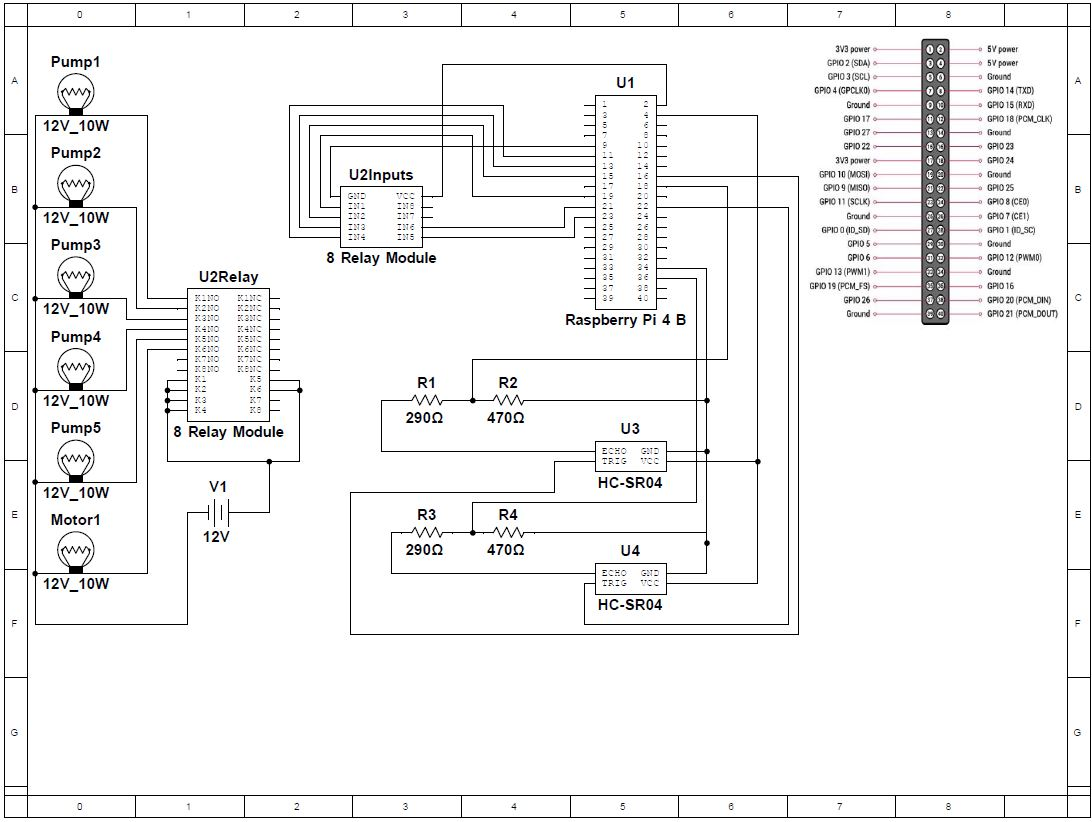
\includegraphics[scale=.75]{Circuit Diagram.JPG}}
    \caption{Circuit Diagram}
    \label{fig}
    \end{figure}
    
The circuit utilizes a raspberry pi to control all logic in the circuit. The pi powers and controls ultrasonic sensors (HC-SR04) to take measurements related to the presence of a cup and how full it is. A relay module is also controlled by the pi's logic to open or close relays that connect an external 12V power supply to all of the pumps and turntable motor in parallel.

\subsection{Circuit Layout}\\ 

    % Figure 2
    \begin{figure}[H]
    \centerline{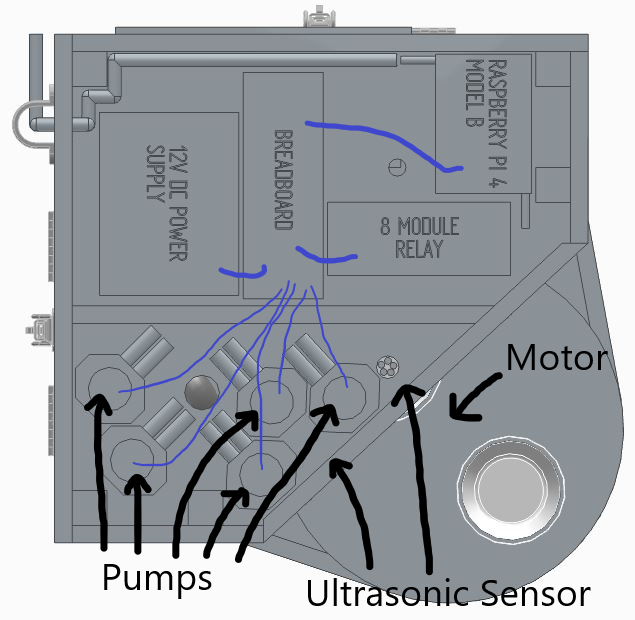
\includegraphics[scale=.5]{Circuit Layout.png}}
    \caption{Circuit Layout}
    \label{fig}
    \end{figure}

The DC motor that is controlling the turntable will be underneath the turntable at it's center. It is not pictured because of this. Similarly the ultrasonic sensors are underneath the enclosure from this view and are also not pictured. They will be positioned as to get readings of the fluid level of the cup, and the presence of a cup, as shown in the diagram below. The connections to the motor and sensors will run up through the enclosure and come out at the hole, connecting to the breadboard.

    % Figure 2
    \begin{figure}[H]
    \centerline{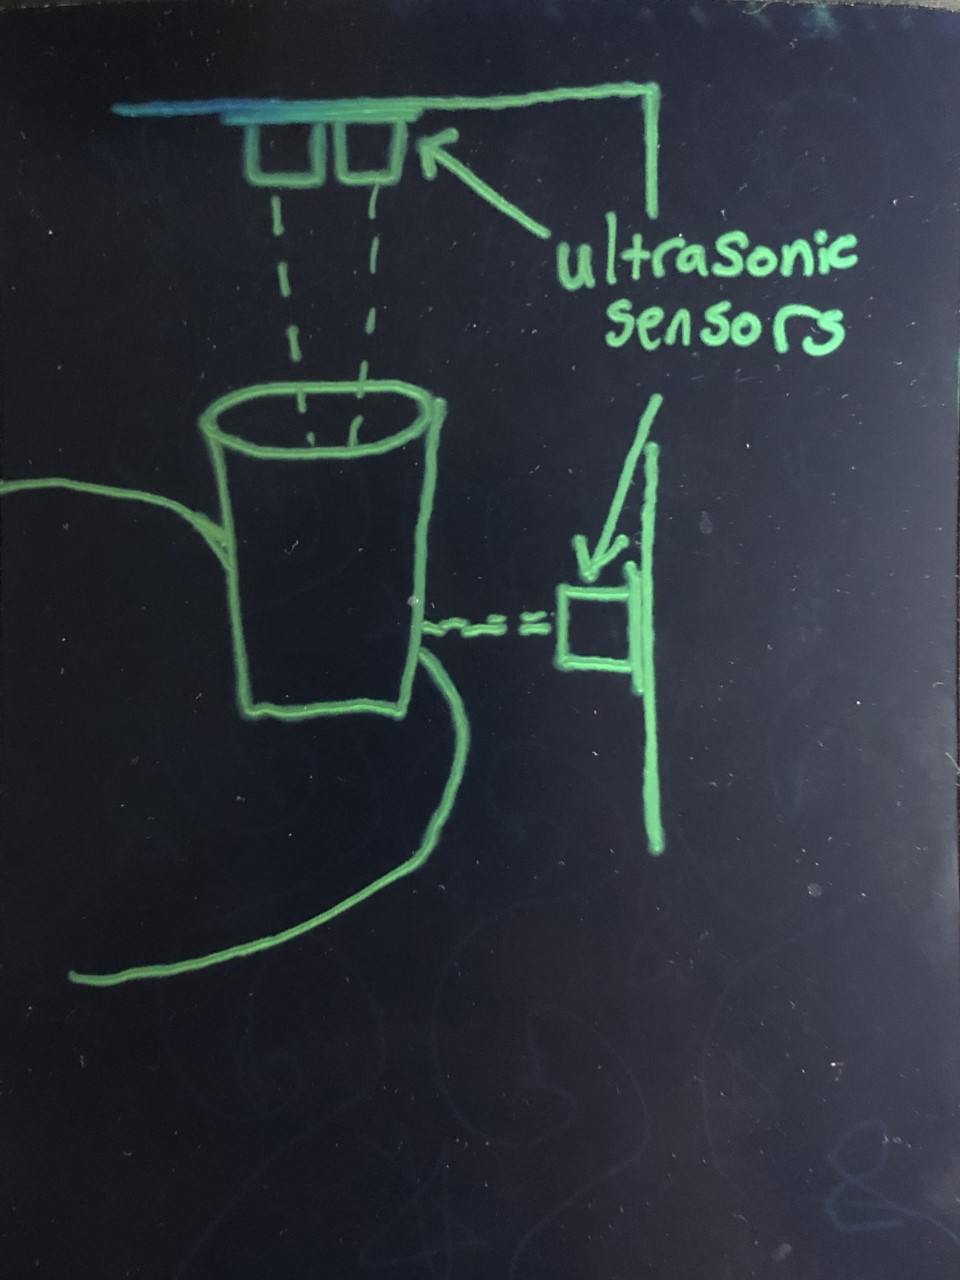
\includegraphics[scale=.3]{Ultrasonic Sensors Diagram.jpg}}
    \caption{Ultrasonic Sensors Diagram}
    \label{fig}
    \end{figure}

\section{Design of Communication Protocols}
The design of communication protocols, involves locally hosting the web application with the final design involving migration to a remote server. Through the help of a internet connected device that is connected to the same network of the raspberry pi, the user will access the Node.js web application through the ip address (or scan from QR code). The database which contains the authentication credentials for the user and drink information will also be locally hosted on the raspberry pi. Upon a user selection of a cocktail on the web app, the Node.js server will execute a python script which will then activate the hardware components to prepare the cocktail. It was decided upon much deliberation, that everything would be hosted locally on the pi for our final product. This would be the easiest way to run scripts on the pi and have the user be able to access the web app when they are in the same setting and close to the Smart Serve machine.

\begin{figure}[H]
    \centerline{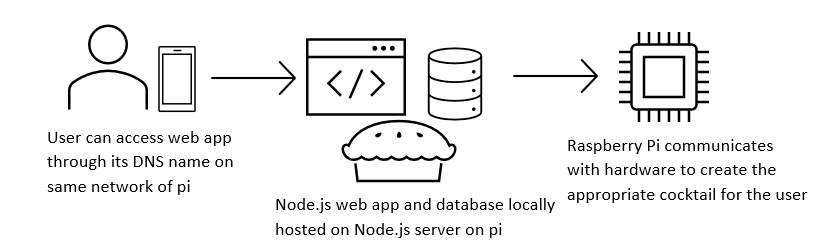
\includegraphics[scale=.5]{initialcommunicationprotocol.png}}
    \caption{Communication Protocol}
    \label{fig}
\end{figure}

\section{Timeline}
The following timeline depicts the given tasks up to the presentation at the Expo. 
\begin{figure}[H]
    \centerline{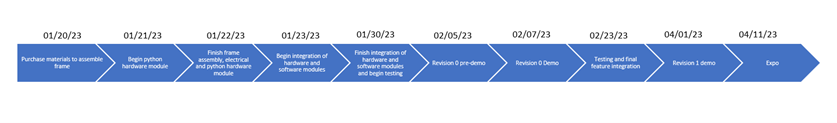
\includegraphics[scale=.9]{timeline.png}}
    \caption{Timeline}
    \label{fig}
\end{figure}


\newpage{}

\section{Appendix}

\begin{figure}[H]
    \centerline{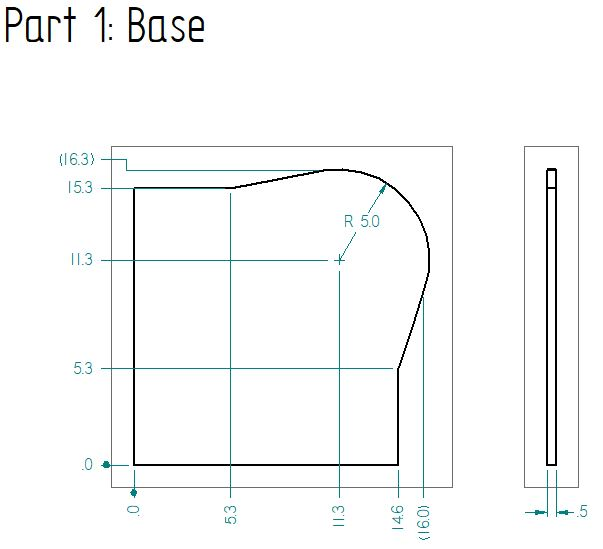
\includegraphics[scale=.5]{Part 1.jpg}}
    \caption{Part 1: Base}
    \label{fig}
\end{figure}

\begin{figure}[H]
    \centerline{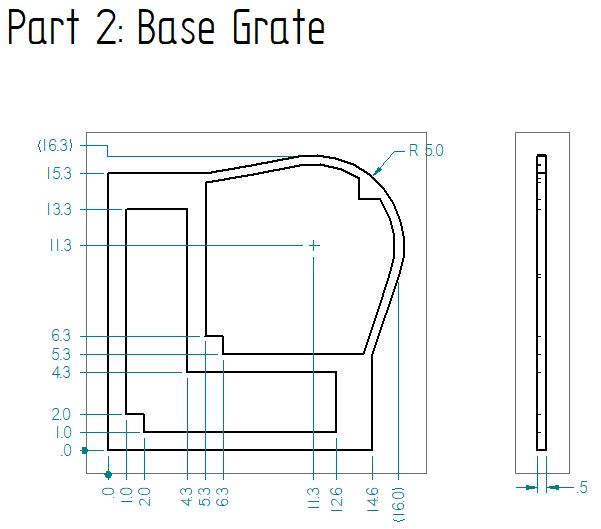
\includegraphics[scale=.5]{Part 2.jpg}}
    \caption{Part 2: Base Grate}
    \label{fig}
\end{figure}

\begin{figure}[H]
    \centerline{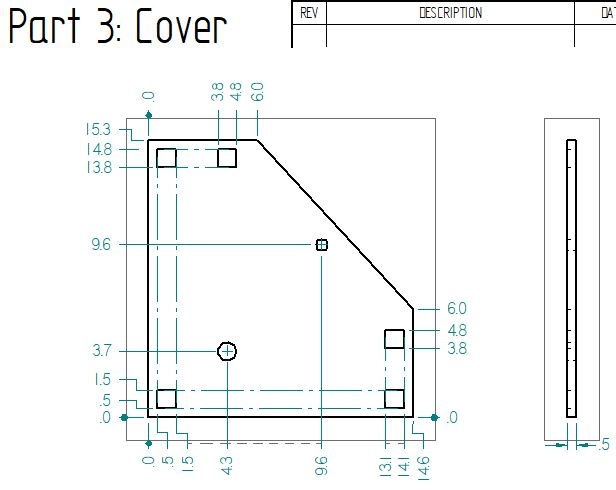
\includegraphics[scale=.5]{Part 3.jpg}}
    \caption{Part 3: Cover}
    \label{fig}
\end{figure}

\begin{figure}[H]
    \centerline{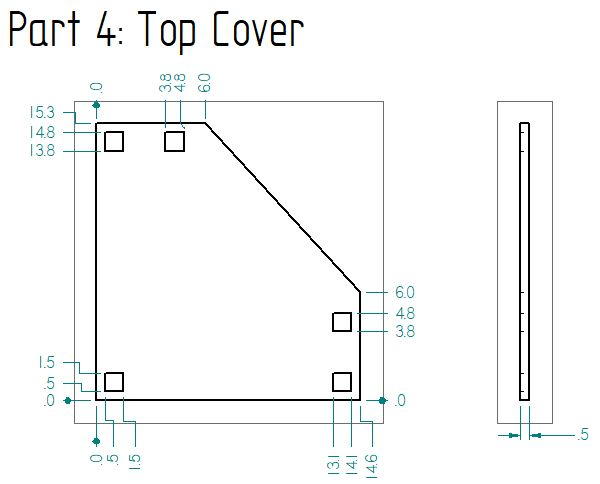
\includegraphics[scale=.5]{Part 4.jpg}}
    \caption{Part 4: Top Cover}
    \label{fig}
\end{figure}

\begin{figure}[H]
    \centerline{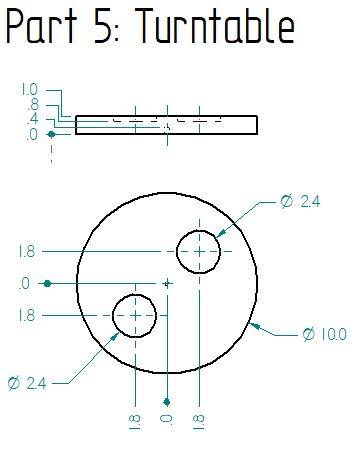
\includegraphics[scale=.5]{Part 5.jpg}}
    \caption{Part 5: Turntable}
    \label{fig}
\end{figure}

\begin{figure}[H]
    \centerline{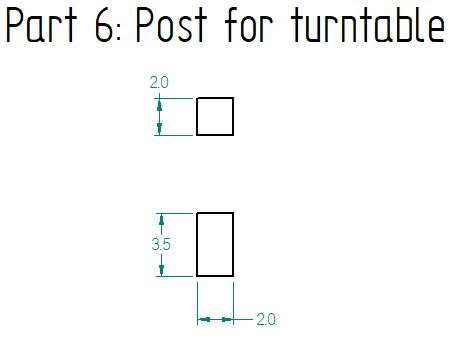
\includegraphics[scale=.5]{Part 6.jpg}}
    \caption{Part 6: Post for turntable}
    \label{fig}
\end{figure}

\begin{figure}[H]
    \centerline{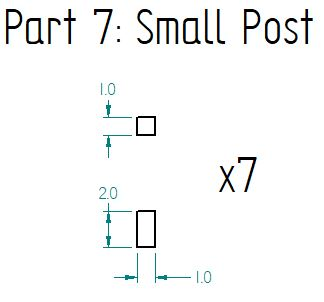
\includegraphics[scale=.5]{Part 7.jpg}}
    \caption{Part 7: Small Post}
    \label{fig}
\end{figure}

\begin{figure}[H]
    \centerline{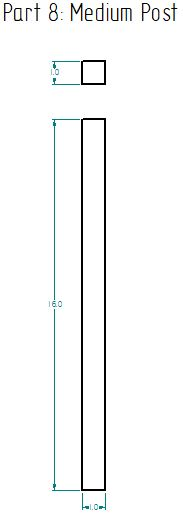
\includegraphics[scale=.5]{Part 8.jpg}}
    \caption{Part 8: Medium Post}
    \label{fig}
\end{figure}

\begin{figure}[H]
    \centerline{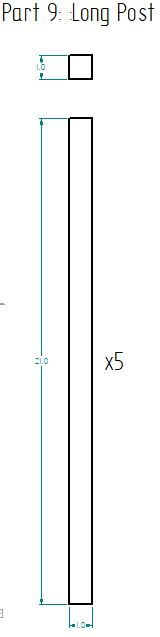
\includegraphics[scale=.5]{Part 9.jpg}}
    \caption{Part 9: Long Post}
    \label{fig}
\end{figure}

\begin{figure}[H]
    \centerline{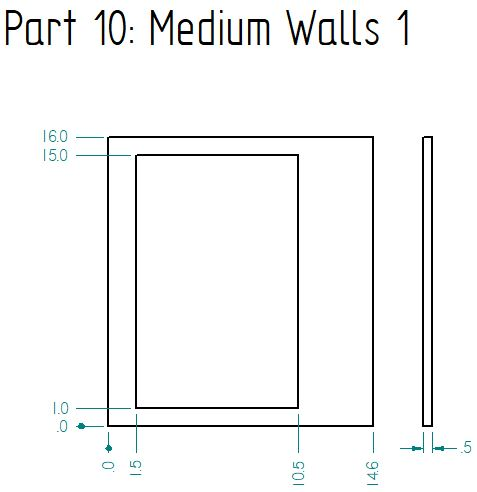
\includegraphics[scale=.5]{Part 10.jpg}}
    \caption{Part 10: Medium Walls 1}
    \label{fig}
\end{figure}

\begin{figure}[H]
    \centerline{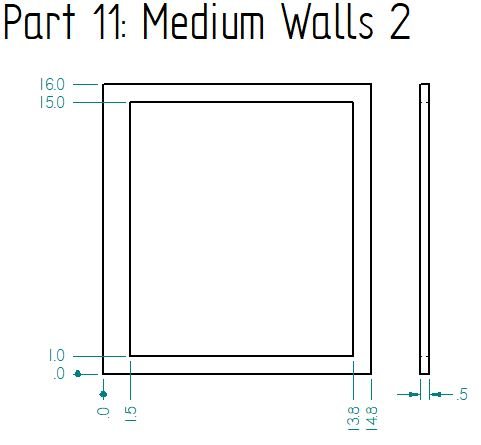
\includegraphics[scale=.5]{Part 11.jpg}}
    \caption{Part 11: Medium Walls 2}
    \label{fig}
\end{figure}

\begin{figure}[H]
    \centerline{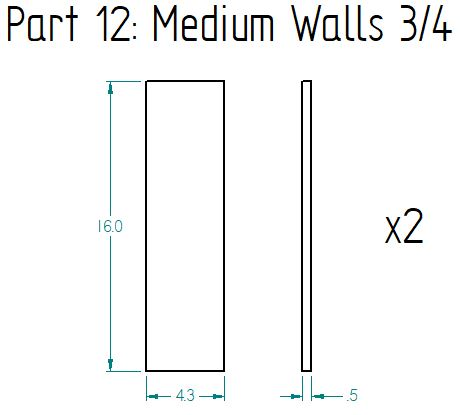
\includegraphics[scale=.5]{Part 12.jpg}}
    \caption{Part 12: Medium Walls 3/4}
    \label{fig}
\end{figure}

\begin{figure}[H]
    \centerline{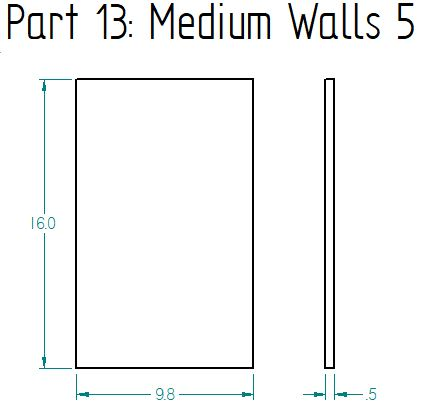
\includegraphics[scale=.5]{Part 13.jpg}}
    \caption{Part 13: Medium Walls 5}
    \label{fig}
\end{figure}

\begin{figure}[H]
    \centerline{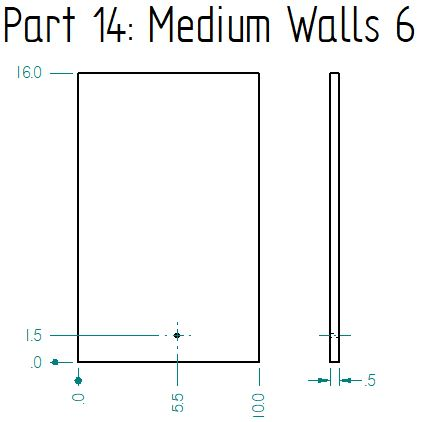
\includegraphics[scale=.5]{Part 14.jpg}}
    \caption{Part 14: Medium Walls 6}
    \label{fig}
\end{figure}

\begin{figure}[H]
    \centerline{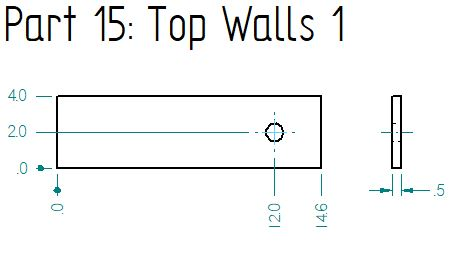
\includegraphics[scale=.5]{Part 15.jpg}}
    \caption{Part 15: Top Walls 1}
    \label{fig}
\end{figure}

\begin{figure}[H]
    \centerline{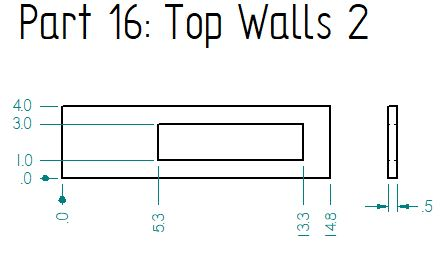
\includegraphics[scale=.5]{Part 16.jpg}}
    \caption{Part 16: Top Walls 2}
    \label{fig}
\end{figure}

\begin{figure}[H]
    \centerline{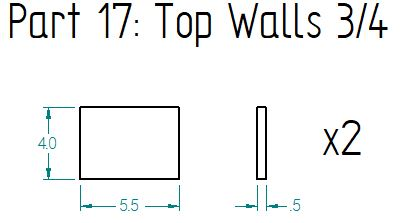
\includegraphics[scale=.5]{Part 17.jpg}}
    \caption{Part 17: Top Walls 3/4}
    \label{fig}
\end{figure}

\begin{figure}[H]
    \centerline{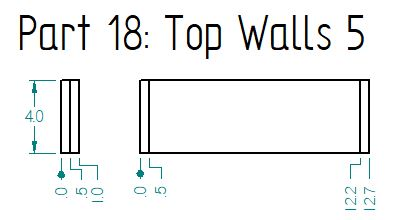
\includegraphics[scale=.5]{Part 18.jpg}}
    \caption{Part 18: Top Walls 5}
    \label{fig}
\end{figure}

\section{Reflection}

%The information in this section will be used to evaluate the team members on the
%graduate attribute of Problem Analysis and Design.  Please answer the following questions:

%\begin{enumerate}
%  \item What are the limitations of your solution?  Put another way, given
%  unlimited resources, what could you do to make the project better? (LO\_ProbSolutions)
%  \item Give a brief overview of other design solutions you considered.  What
%  are the benefits and tradeoffs of those other designs compared with the chosen
%  design?  From all the potential options, why did you select documented design?
%  (LO\_Explores)
%\end{enumerate}

\textbf{Max}\\
It is pretty obvious that time is one of the biggest limitations to our solution. Having strict deadlines for deliverables can be tough, especially when balancing other courses and other commitments. It was tough knowing what parts to order because in some cases we would only have one shot of them working because they took so long to order. This can be very risky, especially if it is a part that is crucial to the design. I think also cost is another limitation to our solution. Since our project is completely self-funded I believe we could've been more innovative in certain design components like for example the frame we could have made out of a plastic or perhaps order stronger pumps. \\

\noindent{}There were a few design options that we had the chance to consider. Firstly, we considered not having a rotating turntable to hold and serve the drinks to the customer. This was due to complexity of the design however, in the end we believed that not having it would eliminate our product from being advantageous to similar cocktail machines that already existed. Furthermore, we considered to switch from a rectangular form to a more rounded edge form along with eliminating a funnel to collect the liquid from the tubes. The benefit of the rectangular form was that it was easier to construct and assemble however, it was found that a more fitted and rounded edge look would reduce weight, wasted space and be more aesthetically pleasing. Finally, removing the use of the funnel although seemed useful to ensure the liquid always landed in the right spot within the cup, caused issues for ultrasonic sensor placement and contamination issues with the mixing of liquids prematurely. \\


\textbf{Sam}\\
One limitation with our solution is that we cannot make every drink available in some stores or bars. While in theory with unlimited resources we would be able to have unlimited ingredients, it isn't feasible to create a bartender robot that can store 200 different ingredients in 2L pop bottles. Another big limitation to our solution is money. Our group doesn't have any funding for this project so price is always a factor when looking at the components that go into the robot. For example, we have to find pumps that produce an acceptable flow rate but within our budget as a group, as opposed to getting the best pumps that can create the drinks as fast as possible. With unlimited resources we could also create a self-cleaning function where the robot could clean itself either after a specific amount of time operating or at the end of each day. \\

\noindent{}One design solution that was considered but not chosen included a cup dropping mechanism. This would allow the user to order a drink on the web application and instead of placing their cup in the cup holder spot, Smart Serve would be able to drop a new cup from a stack of cups onto the turntable disk and simply deliver a finished drink to the user. This was preferred as this would be more automated and require less user intervention. The cup dropping mechanism proved to be quite complicated and was chosen not to be included due to a lack of time and money. Another design solution that was also passed over was a rotating conveyor belt in the shape of a track. This would have potentially allowed up to 5 cups to be on the conveyor belt at once which would speed up the overall process. A drawback to this idea was that it would be more complicated to implement and the benefits of having multiple cups on the conveyor belt wasn't as great when we were limited on how many pumps we could have. As only one cup could be filled at a time, having many cups on the conveyor belt wasn't beneficial. If money wasn't a limiting factor, then we could scale up and fill multiple drinks at once. The solution documented in this document allows us to capture all of the fundamental design requirements while remaining in a reasonable price and time budget.\\


\textbf{Ryan}\\
One big limitation that our solution has is only being able to store 5 different liquids. This limits the amount of drinks that could be created at a specific point in time without replacing the liquid containers with a different drink. With no space constraints, we could store larger quantities of liquids and a greater variety so that our offering is more appealing. Another limitation with our solution is the amount of foam that occurs in the drink when pouring a carbonated drink. This was something that we did not anticipate happening to such an extent, but when testing out pouring with the pumps the foam was excessive. Given more time and money we could play around with ideas such as having two slower pumps to keep the overall flow rate into the cup the same, however the per tube flow rate would be less and the liquid would come out of the tube less quickly. This would likely result in less foam. One final limitation of our solution is the very slow dripping of liquids from the tubes at the cup filling end. This unfortunately adds the chance for small amounts of "contaminant" in drinks. To avoid this we could add motors that control arms which would bring each liquids tube in and out of the pouring area. This would require more space and money for our solution though and did not seem overly feasible. \\

\noindent{}\\ Some designs that I considered were largely centered around sensors. To detect if a cup was present, we could have used a photo detector that detects a thru beam. There was no clear benefit of this design as it would require setting up the sensor to be on both sides of the cup, which was not something that we would be able to do. To determine how full a cup was, we had the option to use a weight scale/load cell. This would determine the weight of a cup and we would be able to tell how full it was that way. The pro of this sensor is that it would not cross contaminate drinks. The con of this sensor is that it would need to be under the cup, and we decided to go with a design that uses a turntable to cycle drinks. This made it unrealistic as we would need at least two of them, and then design our frame to have a way that they could turn freely without getting caught up. So the design would become more complicated. Another sensor that we looked at were etape liquid levels and liquid level floats. These are all easy to use, however the major con is that we cannot have something sitting in the cups as this will easily lead to contamination. Because of these considerations, we went with the ultrasonic sensors to fulfil sensing both the presence of a cup, and how full it is. They are easy to use, will not contaminate drinks, and can be oriented in a way that allows for easy installation, thus simplifying our design. Another design solution that we considered briefly was having the drink run along a conveyor belt and stop at different filling stations to get filled up by one liquid. This would eliminate contamination from the very slight drip of the tubes. The cons of this is that it would make the overall time to create a drink longer, require more space as a compact design like the one we came up with won't work, and we would not have a place to put the next cup until the track is cleared of the previous one. We ended up choosing our current design over this because we valued the time to complete a drink order highly. Having less transportation time for the cup and a cup in place for the next order right away both reduced the overall time for drink delivery.\\


\textbf{David}\\
One major limitation for our solution is the lack of software developer experience in the chosen technology. Given unlimited resources I would purchase better tools and learning materials for the new technology that the  team is working with. Our team consists of one software engineer, one computer engineering, and three mechatronics engineers. The team and I have a strong programming background due to our education and work experience. Even though we have strong programming experience, none of us are extremely experienced with javascript, reactJS, nodeJS, and raspberry Pi’s. This lack of experience forces software development to occur while learning is taking place. This can waste time and resources, and hinders development of new features and stretch goals. This limitation is getting better everyday that we work on the project, but still causes slow development. This limitation also ties into Max's reflection which mentions time as a limitation. Strict deadlines and schoolwork limit time that can be spent learning technology, which can free up much more time for development.\\

\noindent{}\\
One design that we could have selected was a drink dispensing machine with all software embedded in the system. This would include the drink machine itself with a touchscreen feature integrated in the machine. The pros to this would be a convenient and efficient all in one system. All software modules could easily communicate with the hardware. All software could use the same language, shared databases, and shared hardware signals. The cons would be creating a complicated machine. The electrical and mechanical design of the machine would be complex and would be hard to implement in the capstone time frame. The touch screen would attach to the raspberry pi directly along with the rest of the machines components. Another obstacle would be deciding upon the operating systems and the shared software used across both the touch screen, and dispensing hardware. \\

\textbf{Peter}\\
There is a limitation to our solution, that being the complexity of the drinks which can be created. Often, the drinks people choose to order when going to bars are slightly more complex then what can be easily made at home, simply mixing fluids. This may involve adding in sliced fruit or herbs. Given the nature of our solution, primarily focusing on fluids, it eliminates a large pool of exciting drinks which would truly make our ultimate goal successful, to eliminate the need for a human bartender. If given unlimited resources, both money and time, we would find a way to incorporate these more complex drinks.

\\
Another design solution which we considered was a conveyor belt system, a glass moving along a surface stopping at the bottom of ingredient dispensaries as the appropriate amount of fluid poured out. We also considered using a robotic arm to move the glass underneath the bottles for a more quick solution. The main attraction to both these designs was the removal of any potential cross contamination from order to order. Only a single cup would hold the ingredients of an order, as opposed to each drink ingredient being passed through a communal funnel before entering the glass. We chose this design due to its simplicity in nature and our limited budget. A robotic arm would be too complex and time consuming to create. Although a move conveyor belt may not fall into this category, the space required for this design would be far greater than that of our current design. 

\end{document}